% Source: graduate-coursework/Research/Intro_to_Agents/handouts/Part1_Introduction_Installation.tex

\documentclass[border=4pt]{standalone}
\usepackage{amsmath,amssymb}
\usepackage[T1]{fontenc}
\usepackage{graphicx}
\usepackage{lmodern}
\usepackage{tikz}
\usepackage{xcolor}
\usetikzlibrary{shapes.geometric,arrows.meta,positioning,fit,backgrounds,calc}

\definecolor{Garnet}{HTML}{73000A}
\definecolor{DarkGarnet}{HTML}{570008}
\definecolor{Rose}{HTML}{CC2E40}
\definecolor{Atlantic}{HTML}{466A9F}
\definecolor{Congaree}{HTML}{1F414D}
\definecolor{Horseshoe}{HTML}{65780B}
\definecolor{Grass}{HTML}{CED318}
\definecolor{Honeycomb}{HTML}{A49137}
\definecolor{Black90}{HTML}{363636}
\definecolor{Black70}{HTML}{5C5C5C}
\definecolor{Black50}{HTML}{A2A2A2}
\definecolor{WarmGrey}{HTML}{676156}
\definecolor{Sandstorm}{HTML}{FFF2E3}
\definecolor{Azalea}{HTML}{844247}

\tikzset{
    % Sharp corners, no rounded edges
    agentbox/.style={
        rectangle,
        draw=Garnet,
        fill=white,
        thick,
        minimum width=4cm,
        minimum height=1cm,
        align=center,
        font=\small
    },
    agentboxfill/.style={
        rectangle,
        draw=Garnet,
        fill=Sandstorm,
        thick,
        minimum width=4cm,
        minimum height=1cm,
        align=center,
        font=\small
    },
    toolbox/.style={
        rectangle,
        draw=Atlantic,
        fill=white,
        thick,
        minimum width=2.5cm,
        minimum height=0.8cm,
        align=center,
        font=\scriptsize
    },
    categorybox/.style={
        rectangle,
        draw=Congaree,
        fill=Sandstorm,
        thick,
        minimum width=3.5cm,
        minimum height=0.7cm,
        align=center,
        font=\small
    },
    arrow/.style={
        ->,
        >=stealth,
        thick,
        color=Garnet
    },
    dashedarrow/.style={
        ->,
        >=stealth,
        dashed,
        thick,
        color=Atlantic
    }
}

\begin{document}
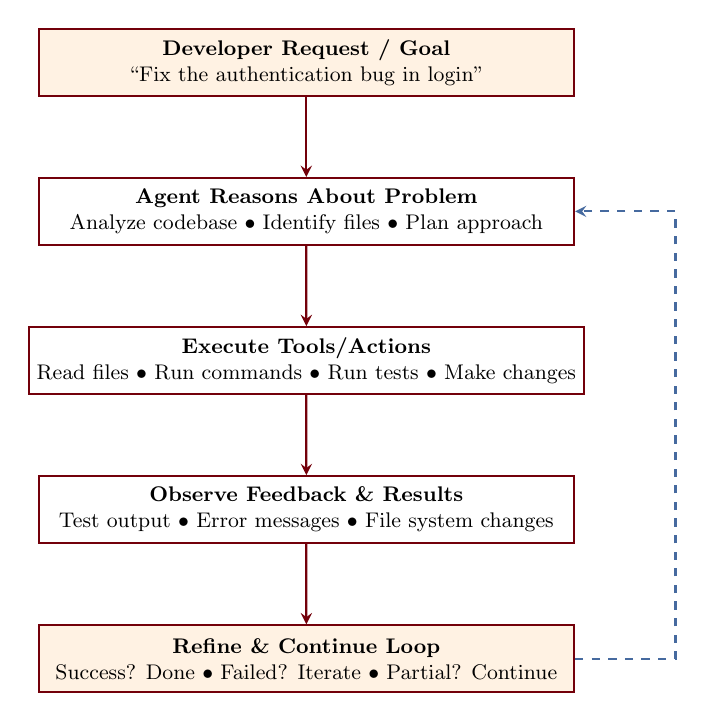
\begin{tikzpicture}[node distance=1.2cm, scale=0.85, transform shape]
            % Developer Request
            \node[agentboxfill, minimum width=8cm] (request) {
                \textbf{Developer Request / Goal}\\
                \small ``Fix the authentication bug in login''
            };

            % Reasoning
            \node[agentbox, below=of request, minimum width=8cm] (reason) {
                \textbf{Agent Reasons About Problem}\\
                \small Analyze codebase $\bullet$ Identify files $\bullet$ Plan approach
            };

            % Execute
            \node[agentbox, below=of reason, minimum width=8cm] (execute) {
                \textbf{Execute Tools/Actions}\\
                \small Read files $\bullet$ Run commands $\bullet$ Run tests $\bullet$ Make changes
            };

            % Observe
            \node[agentbox, below=of execute, minimum width=8cm] (observe) {
                \textbf{Observe Feedback \& Results}\\
                \small Test output $\bullet$ Error messages $\bullet$ File system changes
            };

            % Refine
            \node[agentboxfill, below=of observe, minimum width=8cm] (refine) {
                \textbf{Refine \& Continue Loop}\\
                \small Success? Done $\bullet$ Failed? Iterate $\bullet$ Partial? Continue
            };

            % Arrows (straight lines only)
            \draw[arrow] (request) -- (reason);
            \draw[arrow] (reason) -- (execute);
            \draw[arrow] (execute) -- (observe);
            \draw[arrow] (observe) -- (refine);

            % Loop back arrow (right angle)
            \draw[dashedarrow] (refine.east) -- ++(1.5,0) |- (reason.east);
        \end{tikzpicture}
\end{document}
